\documentclass[12pt, a4paper]{article} %,twoside

\usepackage[literat, microtype, nocolor]{derradeiro}


\setcounter{secnumdepth}{0}

\begin{document}


В результате недавних археологических исследований на острове Paxos оказалось, что существовавший парламент функционировал вопреки приверженности законодателей к странствованиям. Копии записей парламента, хранимые каждым законодателем, были согласованы, несмотря на их частые уходы по важным делам и забывчивость посыльных. Протокол парламента жителей Paxos описывает новый подход к реализации автоматов в распределённой системе.

Представленное было обнаружено недавно за систематизацией материалов в офисе редакции TOCS. Несмотря на древность, главный редактор считал что материал не стоит публикации. Так как автор был занят работой на греческих островах, меня попросили подготовить этот материал.

Автором работы был археолог, который лишь немного интересовался компьютерными науками. К сожалению; ведь даже при условии, что цивилизация Paxon была мало изучена и непонятна, как описывает автор, их законодательная система --- это исключительный пример того, как можно реализовать распределённую систему, работающую в асинхронной среде. Действительно, набор усовершенствований добавленных жителями Paxon в свой протокол оказались не известными в технической литературе.

Автор даёт краткое описание связи Парламента цивилизации Paxon и распределённых вычислений в секции 4. Информатики возможно захотят прочитать эту секцию в первую очередь. И даже раньше они могут обратиться к объяснению алгоритма для информатиков автора Lampson[1996]. Более формально алгоритм описан De Prisco [1997]. Я также добавил дополнительные комментарии о относимости древнего протокола и более современных разработок в конце четвертой секции.

\newpage
\section{Проблема}
\subsection{Остров Paxos}

В начале тысячелетия, эгейский остров Paxos был процветающим торговым центром. Богатство привело к политическому совершенству, и паксоны заменили древнюю теократию парламентской формой правления. Однако торговля всё же стояла на первом месте по отношению к политической ответственности и ни один паксон не горел желанием посвятить свою жизнь парламенту. Парламент должен был функционировать даже при условии, что законодатели постоянно то уходили, то приходили в законодательную палату.

Проблема управления парламентом с частичной занятостью оказывается удивительно схожей с актуальной проблемой создания отказоустойчивых распределённых систем, где законодатели соответствуют процессам, а покидание парламента --- ошибке при обработке. Решение паксонов может заинтересовать информатиков. Я представляю небольшой исторический рассказ о протоколе парламента Paxon, продолжаемый ещё более коротким описанием его отношения к распределённым системам.

Цивилизация Paxon была уничтожена иностранным вторжением, и только недавно археологи начали раскапывать их историю. Наши знания об их парламенте в силу этих обстоятельств достаточно фрагментарны. Несмотря на то, что базовый протокол известен, мы очень плохо осведомлены о многих деталях. Тогда как именно эти детали представляют наибольший интерес. Я возьму ответственность за предположения о том, что же в действительности совершили паксоны.

\subsection{Требования}

Главной задачей парламента заключалась в определении закона (земли), определяемого последовательностью принятых декретов. В современном парламенте бы наняли секретаря для их записи, но среди паксонов не было желающих выполнять эту роль на протяжении всего заседания. Вместо этого, каждый законодатель хранил книгу учёта в которой и делал нумерованные записи принятых декретов. Например, в книге законодателя $\Lambda\iota\nu\chi\partial$ находилась запись:
\[
    155: \textup{Налог на оливки составляет 4 драхмы за тонну}
\]
если они считала, что 155 декрет парламента был принят и устанавливал размер налога на тонну оливок в 4 драхмы. Законодатели писали несмываемыми чернилами так что записи нельзя было изменить. 

Первое требование протокола парламента заключалось в корректности записей в учётных книгах, означающей, что не в каких двух книгах не могло быть противоречивой информации. Если законодатель $\Phi\iota\partial\epsilon\rho$ хранил в своей книге запись 
\[
    132: \textup{Лампы должны использовать только оливковое масло}
\]
то никто другой не мог хранить другую запись для декрета с номером 132. Однако другие законодатели могли под этим номером записи не иметь, если он не знал был ли такой декрет принят.

Соответствие книг учёта было недостаточным, так как они могли быть попросту все пустыми. Должно было быть такое требование, которое бы гарантировало, что декреты в конце концов всё-таки были бы приняты и записаны в книги. В современном парламенте, препятствием к принятию декрета могло быть несогласие среди законодателей. Но такого не было среди паксонов, среди которых преобладала атмосфера взаимного доверия. Законодатели паксонов имели желание принять каждый декрет, выносимый на рассмотрение. Но странствующий уклад жизни был проблемой. Корректность была бы потеряна, если бы одна группа законодателей приняла декрет 
\[ 
    37: \textup{Рисовать на стенах храма запрещено}
\]
а потом ушла на банкет, в то время как другая группа посетила зал заседания и, не зная ничего о том, что произошло, приняла противоречащий закон 
\[
    37: \textup{Свобода художественного самовыражения гарантирована} 
\]

Прогресс не мог быть гарантирован, пока достаточное число законодателей не оставалось в палате достаточное количество времени. Потому как законодатели паксонов не хотели сокращать свои дела не связанные с парламентом, быть уверенным, что когда-нибудь будет принят какой-либо декрет было невозможно. Однако, законодатели желали гарантировать, что находясь в палате, они и их помощники будут действовать без промедлений по всем вопросам парламента. Эта гарантия позволяла вывести протокол парламента, удовлетворяющий следующему условию прогресса:

    Если большинство законодателей\footnote{dd} находились в палате и никто не покидал или входил в палату в течении достаточно долгого периода времени, тогда любой декрет, вынесенный на рассмотрение будет принят и окажется записан во все книги учёта всех законодателей в палате.

\subsection{Допущения}

Требования протокола парламента могли быть удовлетворены только при обеспечении законодателей всеми необходимыми ресурсами. Каждый законодатель получал здоровую книгу для записи декретов, ручку и запас несмываемых чернил. Законодатели могли забывать что они делали после ухода из палаты, поэтому они делали записи о важных задачах в конце книги. Строку в списке декретов нельзя было изменить, но записи в конце можно было (спокойно) вычеркнуть. Для достижения условия прогресса необходимо было, чтобы законодатели могли измерять количество прошедшего времени, и для этого им выдавались простые песочные часы.

Законодатели таскали свои книги всё время и могли всегда прочитать список декретов и любую незачёркнутую запись. Листы книги были изготовлены из тончайшего пергамента, поэтому использовались для самых важных записей. Законодатель мог записать менее важные вещи на листке бумаги, который он мог (или не мог) потерять, когда уходил из парламента.

С той акустикой зала, которая была в палате ораторствовать было совершенно невозможно. Заседающие могли общаться только через посыльных и были снабжены достаточным количеством денег для найма такого их количества, которое им было нужно. Посыльный должен был учесть, что не может исказить сообщение, но ему позволялось забыть, что он только что доставил сообщение и передать его заново. Как и законодатели, посыльные посвящали работе в парламенте только часть времени. Посыльный мог покинуть палату по важному делу, например шестимесячное путешествие, прежде чем доставить сообщение. Он мог также больше никогда не возвращаться, что таким образом делало сообщение потерянным.

Хотя законодатели и посыльные могли приходить и уходить в любое время, в пределах палаты они посвящали всё работе связанной с парламентом. Многие специалисты не верят этому всерьёз, считая эту информацию пропагандой, чтобы изобразить Paxos как землю с более высокими моральными ценностями, чем соседи на востоке. Нечестность, хоть и редко, конечно же была. Однако, в силу того, что ни в одном официальном документе об этом не упоминается, мы имеем слабое представление о то, как они справлялись с нечестным поведением законодателей и посыльных. В секции 3.3.5 будет описаны факты, к которым мы пришли, в проблема.

\section{Синод одного декрета}

Парламент Paxon эволюционировал из раннего церемониального Синода жрецов, который собирался каждые 19 лет для выбора единого, воплощенного в записи декрета. На протяжении многих веков Синод выбирал декрет процедурой взаимного соглашения, требующей присутствия всех членов (жрецов). Но по мере процветания торговли, жрецы во время заседания стали уходить и приходить в палату как получится. В конце концов, старый порядок (протокол) перестал работать и заседание окончилось так и не приняв декрета. Чтобы предотвратить повторения теологической катастрофы, лидеры цивилизации паксон обратились к математикам, чтобы они сформулировали протокол выбора декрета Синода. Требования и допущения протокола были по существу такими же, какие использовались в потом в парламенте, за исключением того, что книга содержала 1 декрет вместо многих. Окончательный протокол Синода описан далее, а протокол парламента в секции 3.

Математики выводили протокол Синода в несколько шагов. Во-первых, они доказали, что протокол, удовлетворяющий набору ограничений будет гарантировать согласованность  и прогресс. \textit{Предварительный протокол} был выведен следом из этого набора ограничений. Ограниченная  версия предварительного протокола,\textit{базовый протокол}\footnote{basic protocol}, гарантировала согласованность, но не прогресс. Завершённый протокол Синода, удовлетворяющий требованиям согласованности и прогресса был получен из базового ввода дополнительных ограничений\footnote{Подробная история создания протокола Синода не известна. Как современные информатики, математики паксонов описывали элегантные, логические выводы, которые не имели ничего общего с тем, как выводят алгоритмы. Однако, известно, что результаты математиков (Теорема 1 и 2 из секции 2.1) действительно предшествовали протоколу. Они были выведены, когда математики, в ответ на запрос создания протокола, пытались доказать, что такого протокола не существует.
}.

\subsection{Результаты математиков}

Декрет Синода выбирался серией пронумерованных \textit{бюллетеней}, где бюллетень был результатом референдума одного декрета. В каждом бюллетене, жрец мог только либо проголосовать за декрет или проигнорировать его\footnote{Как и некоторые современные нации, Paxos не полностью понимали природу Афинской демократии.}. Набор жрецов, называемых \textit{кворумом} ассоциировался с каждым бюллетенем. Бюллетень считался успешным тогда и только тогда, когда каждый жрец в кворуме проголосовал за декрет.  Формально, бюллетень $B$ состоял из 4-х компонентов. (Пока не сказано обратно, \textit{набор} обозначает \textit{конечный набор}\footnote{Несмотря на то, что математики Paxon были очень развитым для того времени, они очевидно не имели знаний о теории множеств. Я взял на себя ответственность в переводе более примитивной нотации в язык современной теории множеств}.)
\begin{table}[h]
\begin{tabular}{ l p{10.5cm}}
    $B_{dec}$ & Декрет (тот, за который проголосовали)\\
    $B_{qrm}$ & Непустой набор жрецов (кворум бюллетеня)\\
    $B_{vot}$ & Набор жрецов (тех, которые голосуют за декрет)\footnote{Только жрецы кворму действительно голосовали, но математики Paxon выяснили, что будет проще убедить людей, что протокол верен, если в их доказательстве они позволят голосовать любому жрецу за любой бюллетень.}\\
    $B_{bal}$ & Номер бюллетеня
\end{tabular}
\end{table}

Бюллетень $B$ называелся \textit{успешным} титтк $B_{qrm} \subseteq B_{vot}$ так, что успешный бюллетень соответствует тому, за который проголосовали все члены кворума.

Номера бюллетеней выбирались из бесконечного упорядоченного набора чисел. Если $B_{bal}' > B_{bal}$, тогда бюллетень $B'$ назвался более поздним, чем $B$. Однако, это никак не отражало тот порядок, в котором бюллетени обрабатывались; более поздний бюллетень мог быть обработан перед ранним.

Математики Paxon определили 3 ограничения над набором $\mathcal{B}$ бюллетеней и далее показали, что обеспечивается согласованность, а прогресс может иметь место, если обрабатываемый набор бюллетеней соответствовал этим ограничениям. Первые два ограничения были простыми; они могут быть сформулированы неформально следующим образом.
\begin{table}[h]
\begin{tabular}{l p{10.5cm}}
    $B1(\mathcal{B})$ & Каждый бюллетень в $\mathcal{B}$ обладает уникальным номером.\\
    $B2(\mathcal{B})$ & Кворумы любых двух бюллетеней в $\mathcal{B}$ включают хотя бы одного общего жреца.
\end{tabular}
\end{table}

Третье ограничение было более сложным. Один манускрипт Paxon содержал следующее, достаточно запутанное утверждение.
\begin{table}[h]
\begin{tabular}{l p{10.5cm}}
    $B3(\mathcal{B})$ & Для каждого бюллетеня $B$ в $\mathcal{B}$, если любой жрец в кворуме голосовал за \textit{предыдущий} бюллетень в $\mathcal{B}$, тогда декрет $B$ эквивалентен декрету последнего бюллетеня из ранних бюллетеней. 
\end{tabular}
\end{table}

Интерпритация этого загадочного текста облегчалась манускриптов, изображённым на рисунке 1, который иллюстрирует условие $B3(\mathcal{B})$ с набором $\mathcal{B}$ из пяти бюллетеней для Синода, состоящего из пяти жрецов $A$, $B$, $\Gamma$, $\Delta$ и $E$. Этот набор $\mathcal{B}$ состоящий из пяти бюллетеней, где для каждого бюллетеня, набор голосующих --- подмножество жрецов кворума, чьи имена заключены в рамки. Например, номер бюллетеня 14 содержал декрет $\alpha$, кворум, состоящий из трёх жрецов и набор из двух голосующих. Условие $B3(\mathcal{B})$ имело вид <<для каждого $B$ в $\mathcal{B}$: $\ldots$>>, где <<$\ldots$>> --- это условие бюллетеня $B$. Условия пяти бюллетеней $B$ Рисунка 1 следующие.

%\begin{figure}[h]
% \centering
%    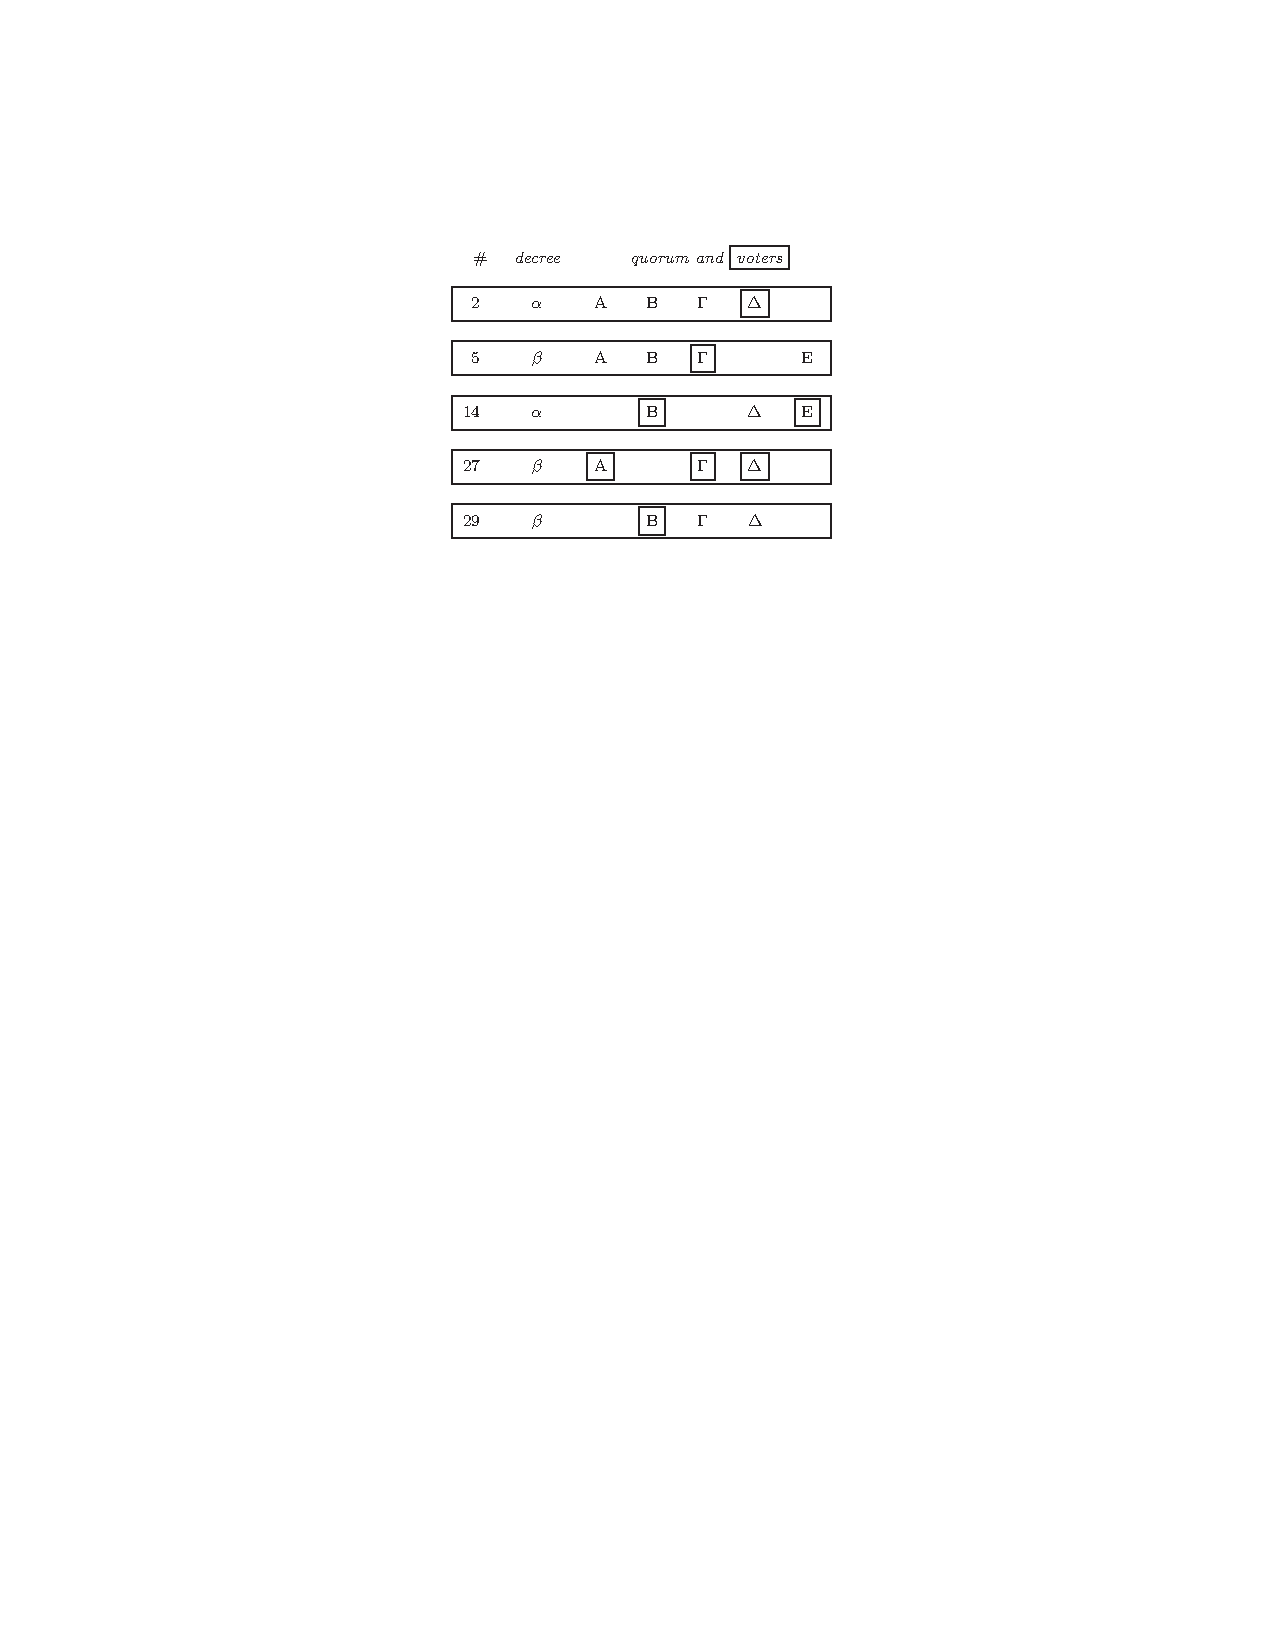
\includegraphics[width=0.6\textwidth]{images/Paxon-manuscript.pdf}
%\end{figure}

\begin{itemize}
    \item[2.] Бюллетень с номером 2 --- самый ранний бюллетень, поэтому его ограничение тривиальное и равно истине.
    \item[5.] Ни один из членов кворума бюллетеня под номером 5 не голосовал за ранний, так что ограничение также просто равное истине.
    \item[14.] Единственный член бюллетеня 14, который голосовал за предыдущие это $\Delta$, проголосовавший за номер 2, так что условие требует того, чтобы декрет 14 бюллетеня был также декретом 2-ого.
    \item[27.] (Успешный бюллетень.) Члены кворума 27-ого бюллетеня: $A$, $\Gamma$ и $\Delta$. Жрец $A$ не голосовал за ранние бюллетени, единственный ранний бюллетень за который голосовал $\Gamma$ это 5-ый, а $\Delta$ оставил голос за 2. Последний из этих двух бюллетений --- пятый, таким образом согласно ограничению декрет 27-ого бюллетеня должен совпадать с 5-ым.
    \item[29.] Члены кворума бюллетеня 29: $B$, $\Gamma$ и $\Delta$. $B$ уже один раз проголосовал за 14, жрец $\Gamma$ за 5 и 27, а $\Delta$ голосовал за 2-й и 27-й. Самый поздний из четырёх бюллетений --- 27, поэтому условие требует, чтобы 29 декрет совпадал с 27.
\end{itemize}


Чтобы утверждать $B1(\mathcal{B}) - B3(\mathcal{B})$ формально требуется дополнительная нотация (определения). \textit{Голос} $v$ был определён как элемент, состоящий из трёх компонетов: жреца $v_{pst}$, бюллетеня $v_{bal}$ и декрета $v_{dec}$. Он представляет голос осуществлённый жрецом $v_{pst}$ за декрет $v_{dec}$ в бюллетене $v_{bal}$. Паксоны также ввели $null$ голоса, такие, что $v_{bal}=-\infty$ и $v_{dec}=\mathrm{BLANK}$, где $-\infty < b < \infty$ для любого номера бюллетеня $b$ и $\mathrm{BLANK}$ не являющийся декретом. Для любого жреца $p$, они ввели $null_p$ как уникальный голос $v$, где $v_{pst}=p$.

Математики Paxon определили полное упорядочение над множеством всех голосов, но часть манускрипта, содержащая эту информацию была утеряна. Сохранившийся фрагмент подсказывает, что для любого голоса $v$ и $v'$, при условии, что $v_{bal} < v_{bal}'$ выполняется $v < v'$. Нет информации о том, в каком порядке идут $v$ и $v'$, если $v_{bal} = v_{bal}'$.

Для любого множества $\mathcal{B}$, множество $Votes(\mathcal{B})$ голосов в $\mathcal{B}$ было определено состоящим из голосов $v$, таких, что $v_{pst} \in B_{vot}? v_{bal} = B_{bal}$ и $v_{dec} = B_{dec}$ для некоторых $B \in \mathcal{B}$. Если $p$ --- жрец, а $b$ номер бюллетеня или $\pm \infty$, тогда $MaxVote(b, p, \mathcal{B})$ было определено как максимальный голос из $Votes(\mathcal{B})$ совершённый $p$ c $v_{bal} < b$, или было равным $null_p$, если такого голоса не существовало. Так как $null_p$ меньше чем любой реально осуществлённый голос $p$, то $MaxVote(b,p, \mathcal{B})$ --- это максимальный голос из множества:
\[  
    \{v \in Votes(\mathcal{B}) : (v_{pst} = p) \land (v_{bal} < b)\} \cup \{null_p\}
\]
Для любого непустого множества жрецов $Q$, $MaxVote(b, Q, \mathcal{B})$ был определён равным как максимум всех голосов $MaxVote(b, p, \mathcal{B})$ c $p$ d $Q$.

Ограничения  $B1(\mathcal{B}) - B3(\mathcal{B})$ утверждаются формально следующим образом:
\begin{align*}
    &B1(\mathcal{B}) \overset{\Delta}{=} \forall B, B' \in \mathcal{B} : (B \neq B') \Rightarrow (B_{bal} \neq B_{bal}') \\
    &B2(\mathcal{B}) \overset{\Delta}{=} \forall B, B' \in \mathcal{B} : B_{qrm} \cap B_{qrm}' \neq \emptyset \\
    &B3(\mathcal{B}) \overset{\Delta}{=} \forall B \in \mathcal{B} : (MaxVote(B_{bal}, B_{qrm}, \mathcal{B})_{bal} \neq - \infty) \Rightarrow \\
    &(B_{dec} MaxVote(B_{bal}, B_{qrm}, \mathcal{B})_{dec}) \\
\end{align*}
Несмотря на то, что определение $MaxVote$ зависит от порядка голосов, $B1(\mathcal{B})$ влечёт за собой то, что $MaxVote(b, Q, \mathcal{B})_{dec}$ независит от того, в каком порядке идут голоса с эквивалентными номерами бюллетеней.

Чтобы показать, что согласованность является следствием этих ограничений, Паксоны в первую очеред показали, что при условиях $B1(\mathcal{B}) - B3(\mathcal{B})$, если $B$ в $\mathcal{B}$ успешен, то любой поздний бюллетень из $\mathcal{B}$ относится к одному и тому же декрету, что и $B$.

\begin{lemma}
Если $B1(\mathcal{B})$, $B2(\mathcal{B})$ и $B3(\mathcal{B})$ ограничения в силе, тогда
\[
    ((B_{qrm} \subseteq B_{vot}) \land (B_{bal}' > B_{bal})) \Rightarrow (B_{dec}' = B_{dec})
\]
\end{lemma}
\begin{lemmaproof}
Для любого бюллетеня $B$ в $\mathcal{B}$, пусть $\Psi(B, \mathcal{B})$ будет подмножеством бюллетеней в $\mathcal{B}$ более поздних, чем $B$ для декрета отличного от $B$:
\[
    \Psi(B, \mathcal{B}) \overset{\Delta}{H} \{B' \in \mathcal{B} : (B_{bal}' > B_{bal}) \land (B_{dec}' \neq B_{dec})\}
\]

Чтобы доказать лемму, достаточно показать, что если $B_{qrm} \subseteq B_{vot}$, тогда $\Psi(B, \mathcal(B))$ --- пустое множество. Паксоны использовали доказательство от противного приведённое ниже\footnote{Математики Паксонов всегда предоставляли аккуратные, структурированние доказательства важных теорем. Они были не такими хитроумными как современные математики, которые могут опустить многие детали и не сделать ошибку в доказательствах размером с абзац.}.
\begin{enumerate}
    \item Выберем $C \in \Psi(B, \mathcal{B})$ такое, что $C_{bal} = min \{B_{bal}' : B' \in \Psi(B, \mathcal(B))\}$. \\
          \textsc{Proof}: $C$ существует потому, что $\Psi(B, \mathcal{B})$ непустое и конечное.
    
    \item $C_{bal} > B_{bal}$\\
          \textsc{Proof}: Исходя из пункта 1 и определения $\Psi(B, \mathcal{B})$.

    \item $B_{vot} \cap C_{qrm} \neq \emptyset$\\
          \textsc{Proof}: Следует из  $B2(\mathcal{B})$ и гипотезы, что $B_{qrm} \subseteq B_{vot}$.
    
    \item $MaxVote(C_{bal}, C_{qrm}, \mathcal{B}) \geqslant B_{bal}$\\
          \textsc{Proof}: Из 2, 3 и определения $MaxVote(C_{bal}, C_{qrm}, \mathcal{B})$.

    \item $MaxVote(C_{bal}, C_{qrm}, \mathcal{B}) \in Votes(\mathcal{B})$\\
          \textsc{Proof}: Из 4, которое влечёт, что $MaxVote(C_{bal}, C_{qrm}, \mathcal{B})$ не $null$ голос и определения  $MaxVote(C_{bal}, C_{qrm}, \mathcal{B})$.

    \item $MaxVote(C_{bal}, C_{qrm}, \mathcal{B})_{dec} = C_{dec}$.\\
          \textsc{Proof}: Из 5 и $B3(\mathcal{B})$.

    \item $MaxVote(C_{bal}, C_{qrm}, \mathcal{B})_{dec} \neq B_{dec}$.\\
          \textsc{Proof}: Из 6, 1 и определения $\Psi(B, \mathcal{B})$.

    \item $MaxVote(C_{bal}, C_{qrm}, \mathcal{B})_{bal} > B_{bal}$.\\
          \textsc{Proof}: Из 4, так как 7 и $B1(\mathcal{B})$ влекут \\
          $MaxVote(C_{bal}, C_{qrm}, \mathcal{B})_{bal} \neq B_{bal}$.

    \item $MaxVote(C_{bal}, C_{qrm}, \mathcal{B}) \in Votes(\Psi(B, \mathcal{B}))$.\\
          \textsc{Proof}: Из 7, 8, b определения $\Psi(B, \mathcal{B})$.

    \item $MaxVote(C_{bal}, C_{qrm}, \mathcal{B})_{bal} Б С_{bal}$.\\
          \textsc{Proof}: По определению $MaxVote(C_{bal}, C_{qrm}, \mathcal{B})_{bal}$.
    
    \item Противоречие\\
          \textsc{Proof}: Из 9, 10 и 1.
\end{enumerate}
\end{lemmaproof}

С помощью этой леммы было просто показать, что если выполняются $B1(\mathcal{B}) - B3(\mathcal{B})$, то любые два успешных бюллетеня соответствуют одному декрету.
\begin{theorem}
Если $B1(\mathcal{B})$, $B2(\mathcal{B})$ и $B3(\mathcal{B})$ в силе, то
\[
    ((B_{qrm} \subseteq B_{vot}) \land (B_{qrm}' \subseteq B_{vot}')) \Rightarrow (B_{dec}' = B_{dec})
\]
для любого $B$, $B'$ в $\mathcal{B}$.
\end{theorem}
\begin{theoremproof}
Если $B_{bal}' = B_{bal}$, тогда $B1(\mathcal{B})$ влечёт $B' = B$. Если $B_{bal}' \neq B_{bal}$, тогда утверждение теоремы выводится непосредственно из леммы.
\end{theoremproof}

Паксоны доказали теорему, полагая, что если в Палате достаточно жрецов, то возможен успешный бюллетень при ограничениях $B1-B3$. Хотя это не гарантировало прогресс, доказательство показывало, что протокол опирающийся на ограничения $B1-B3$ не приведёт к мёртвой блокировке.

\begin{theorem}
Пусть $b$ --- номер бюллетеня и $Q$ множество жрецов такое, что $b > B_{bal}$ и $Q \cap B_{qrm} \neq \emptyset$ для любых $B \in \mathcal{B}$. Если $B1(\mathcal{B})$, $B2(\mathcal{B})$ и $B3(\mathcal{B})$ действуют, тогда существует бюллетень $B'$ с $B_{bal}' = b$ и $B_{qrm}' = B_{vot}' = Q$ такой, что $B1(\mathcal{B} \cup \{B'\})$, $B2(\mathcal{B} \cup \{B'\})$ и $B3(\mathcal{B} \cup \{B'\})$ в силе.
\end{theorem}
\begin{theoremproof}
Условие $B1(\mathcal{B} \cup \{B'\})$ следует из $B1(\mathcal{B})$, выбора $B_{bal}'$, и допущения о $b$. Условие  $B2(\mathcal{B} \cup \{B'\})$ следует из  $B2(\mathcal{B})$, выбора $B_{qrm}'$ и допущения о $Q$. Если $MaxVote(b, Q, \mathcal{B})_{bal} = - \infty$, тогда пусть $B_{dec}'$ будет любым декретом, иначе равным $MaxVote(b, Q, \mathcal{B})_{dec}$. Условие $B3(\mathcal{B} \cup \{B'\})$ тогда следует из $B3(\mathcal{B})$.
\end{theoremproof}

Паксоны вывели \textit{предварительный протокол} из требования, что $B1(\mathcal{B}) - B3(\mathcal{B})$ выполняются, где $\mathcal{B}$ был множеством всех бюллетеней, которые были обработаны или обрабатывались в данный момент. Определение протокола говорило как множество $\mathcal{B}$ изменялось, но само оно никогда явно не рассчитывалось. Паксоны относились к $\mathcal{B}$ как к элементу, о котором дозволено знать только богам, так, что оно не было известно ни одному смертному.

Каждый бюллетень инициировался (создавался) жрецом, который выбирал его номер, декрет и кворум. Каждый жрец кворума затем выбирал голосовать за бюллетень или нет. Правила определявшие, как инициатор выбирал номер бюллетеня, декрет и кворум и как жрец решал голосовать или нет выводились непосредственно из необходимости удовлетворять ограничениям $B1(\mathcal{B}) - B2(\mathcal{B})$.

Чтобы поддерживать $B1$, каждый бюллетень должен был получить уникальный номер. Запоминая (то какие записи в книге учёта) какие бюллетени были ранее инициированы, жрец мог легко избежать инициации двух разных бюллетеней с одним и тем же номером. Чтобы не допустить инициации бюллетеня с одним номером разными жрецами, множество возможных номеров было между ними разделено. Хотя неизвестно как это происходило, очевидным способом было бы считать номер бюллетеня парой из целого числа и имени жреца, используя лексикографический порядок, где
\[
    (13, \Gamma\rho\alpha\iota) < (13, \Lambda\iota\nu\delta\epsilon\iota) < (15, \Gamma\rho\alpha\iota)
\]
так как $\Gamma$ предшествует $\Lambda$ в алфавите Паксонов. В любом случае, известно, что каждый жрец имел неограниченное множество номеров бюллетеней, выделенных для него.

Чтобы поддержать $B2$, кворум бюллетеня выбирался так, чтобы содержать $\mu\alpha\delta\sigma\omega\rho\iota\tau\iota'\delta\epsilon\tau$ жрецов. Первоначально, $\mu\alpha\delta\sigma\omega\rho\iota\tau\iota'\delta\epsilon\tau$ означало обычное большинство. Позднее выяснилось, что толстые жрецы были менее мобильны и тратили больше времени в Палате, чем худые, так, что $\mu\alpha\delta\sigma\omega\rho\iota\tau\iota'\delta\epsilon\tau$ стало означать любое множество жрецов, чья общая масса была больше половины всех жрецов, нежели просто большинство. Когда группа худых жрецов пожаловалась на то, что это несправедливо, действительные веса заменили на символические, основанные на записи о посещяемости жреца. Первичное требование для $\mu\alpha\delta\sigma\omega\rho\iota\tau\iota'\delta\epsilon\tau$ было то, что любые два множества, содержащие $\mu\alpha\delta\sigma\omega\rho\iota\tau\iota'\delta\epsilon\tau$ включали хотя бы одного общего жреца. Чтобы удовлетворить $B2$ жрец инициировал бюллетень $B$, выбирая $B_{qrm}$ как множество большиства.

Условие $B3$ требовало, что при условии $MaxVote(b, Q, \mathcal{B})_{dec}$ не равно \textsc{BLANK}, бюллетень с номером $b$ и кворум $Q$ должны иметь декрет $MaxVote(b, Q, \mathcal{B})_{dec}$. Если $MaxVote(b, Q, \mathcal{B})_{dec}$ был равен \textsc{BLANK}, тогда бюллетен мог соответствовать любому декрету. Обеспечивая выполнение $B3(\mathcal{B})$, до инициирования нового бюллетеня с номером $b$ и кворумом $Q$ жрец $p$ должен был найти $MaxVote(b, Q, \mathcal{B})_{dec}$. Для этого ему необходимо найти $MaxVote(b, q, \mathcal{B})$ для каждого жреца $q$ в $Q$.

Вспоминая, что $MaxVote(b, Q, \mathcal{B})$ --- голос с наибольшим номером, меньшим чем $b$ среди всех голосов осуществлённых жрецом $q$ или $null_p$ если $q$ не голосовал ни за один бюллетен с номером меньшим $b$. Жрец $p$ получал $MaxVote(b, q, \mathcal{B})$ из $q$ обмениваясь сообщениями. По этому причине, первые два шага протокола для вывода одного бюллетеня инициированного $p$ следующие\footnote{Жрецы $p$ и $q$ могли быть одним и тем же человеком. Для упрощения, протокол описан с $p$ посылающим сообщения самому себе в таком случае. В реальности, жрецы могли говорить сами с собой и без посыльных.}:

\begin{enumerate}
    \item Жрец $p$ выбирает новый номер бюллетеня и отправляет \\$NextBallot(b)$ сообщение множеству жрецов.
    \item Жрец $q$ отвечает на получение $NextBallot(b)$ сообщением $LastVote(b, v)$ жрецу $p$, где $v$ голос с максимальным номером бюллетеня меньшим $b$, который $q$ совершил, либо сообщением с $null_p$, если он не голосовал ни за один бюллетень, номеро которого меньше $b$.
\end{enumerate}

Жрец $q$ должен был использовать записи с последней страницы своей книги, чтобы запомнить какие голоса он уже совершил.

Когда $q$ посылает сообщение $LastVote(b, v)$, $v$ равно $MaxVote(b, q, \mathcal(B))$. Но множество бюллетеней $\mathcal{B}$ изменяется когда инициируется новый бюллетень и когда кто-то отдаёт свой голос. Так как $p$ собирается использовать $v$ как значение $MaxVote(b, q, \mathcal{B})$ при выборе декрета, для выполнения $B3(\mathcal{B})$ требуется, чтобы $MaxVote(b, q, \mathcal(B))$ не изменился после того, как $q$ отправил $LastVote(b, v)$. Чтобы предотвратить изменение $MaxVote(b, q, \mathcal(B))$, $q$ не должен более голосовать за бюллетени с номерами между $v_{bal}$ и $b$. Отправляя $LastVote(b, v)$ сообщение, $q$ даёт обещание не делать таких голосов. (Для того, чтобы его сдержать жрецу может понадобится записать необходимую информацию в книгу.)

Следующие 2 шага протокола (начатые жрецом $p$ на первом шаге):
\begin{enumerate} \setcounter{enumi}{2}
    \item После получения сообщения $LastVote(b, v)$ от большинства жрецов множества $Q$, жрец $p$ инициирует новый бюллетень с номером $b$, кворумом $Q$ и декретом $d$, где декрет $d$ выбирается так, чтобы удовлетворить $B3$. Затем он записывает бюллетень в конец книги учёта и посылает сообщение $BeginBallot(b, d)$ каждому жрецу в $Q$.
    \item В ответ на $BeginBallot(b, d)$, жрец $q$ принимает решение о голосе за бюллетень с номером $b$. (Он может не отдать голоса, если это будет противоречить обещанию, связанному с сообщением $LastVote(b', v')$ для другого бюллетеня.) Если $q$ решает проголосовать за $b$, тогда он отправляет сообщение $Voted(b, q)$ жрецу $p$ и записывает голос в конец своей книги.
\end{enumerate}

Выполнение шага 3 подразумевает добавление $B$ в $\mathcal{B}$, где $B_{bal} = b$, $B_{qrm} = Q$, $B_{vot} = \emptyset$ (никто более не голосовал за данный бюллетень) и $B_{dec} = d$. На шаге 4, если жрец $q$ голосует за бюллетень, тогда выполнение этого шага подразумевает измениение множества бюллетеней $\mathcal{B}$ добавлением $q$ в множество проголосовавших $B_{vot}$ бюллетеня $B \in \mathcal{B}$.


У жреца есть выбор не голосовать на 4 шаге, если это будет противоречить его предыдущему обещанию. По правде говоря, все шаги протокола не обяхяательные. Например, жрец $q$ может проигнорировать $NextBallot(b)$ сообщение, вместо выполнения 2-ого шага. Невозможность предпринять действия может предотвратить достижения прогресса, но не может привести к несогласованному состоянию, так как $B1(\mathcal{B}) - B3(\mathcal{B})$ не станут ложными. Так единственным эффектом неполучения сообщения будет отсутствие полезных действий, потеря сообщения также не приведёт к несогласованности. Следовательно, протокол гарантирует согласованность даже если жрец покидает палату или сообщение теряет.

Поулчение нескольких копий сообщения может повлечь совершение повторных действий. За исключением шага 3, совершение повторного действия не ни на что не влияет. Например, отправление нескольких $Voted(b, q)$ на 4-ом шаге имеет тот же эффект, что и отправление одного. Повторение шага 3 предотвращается записью в конце книги при выполнении. Так, согласованность сохраняется даже если и посыльный приносит то же сообщение несколько раз.

Шаги протокола 1--4 полностью описывают инициацию бюллетеня и голосование за него. Всё что остаётся, это определить результат голосования и сделать объявление, когда какой-либо декрет выбран. Вспомним, что бюллетень успешен тогда и только тогда, когда каждый жрец кворума проголосовал. Декрет успешного бюллетеня есть декрет выбранный Синодом. Оставшаяся часть протокола:
\begin{enumerate} \setcounter{enumi}{4}
    \item Если $p$ получил сообщение $Voted(b, q)$ от каждого $q$ из $Q$ (кворума бюллетеня $b$), тогда он записывает $d$ (соответствующий декрет бюллетеня) в свою книгу и посылает $Success(d)$ сообщение каждому жрецу.

    \item По получению сообщения $Success(d)$, жрец вносит декрет $d$ в свою книгу.
\end{enumerate}

Шаги 1--6 описывают как обрабатывается один бюллетень. Предварительный протокол позволяет любому жрецу инициировать бюллетень в любое время. Каждый шаг согласуется с $B1(\mathcal{B}) - B3(\mathcal{B})$ так, что протокол в целом им удовлетворяет. В виду того, что жрецы заносят в книгу декрет только успешного бюллетеня, из Теоремы 1 следует, что книги жрецов всегда согласованы. Протокол не касается вопроса достижения прогресса.

На шаге 3, если декрет $d$ определяется условием $B3$, возможно, что декрет уже записан в книгу какого-либо жреца. Этот жрец может не входить в кворум $Q$: он может не находится в Палате. Следовательно, согласованность не может быть гарантирована, если шаг 3 позволяет большую свободу в выборе $d$.

\subsection{Базовый протокол}

В предварительном протоколе, жрец должен был записать (i) номер всех инициированных им бюллетеней, (ii) каждый отданный им голос и (iii) каждое посланное $LastVote$ сообщение. Вести наблюдение за всей этой информацией должно было быть сложным для занятых жрецов. Паксоны по этой причине ограничили предварительный протокол для получения более практичного \textit{базового протокола}, в котором каждый жрец $p$ должен был поддерживать в конце книги учёта только следующую информацию:
\begin{itemize}
    \item[]lastTried[p] Номер последнего бюллетеня, который $p$ пытался инициировать, или $-\infty$ если таких не было.
    \item[]prevVote[p] Голос $p$ за бюллетень с максимальным номером из бюллетеней, за которые голосовал жрец, либо $-\infty$ если он никогда не голосовал.
    \item[]nextBal[p] Максимальный номер $b$ для которого $p$ послал $LastVote(b, v)$, либо $-\infty$, если он никогда не посылал таких сообщений.
\end{itemize}

Шаги 1--6 предварительного протокола описывают как обрабатывался один бюллетень инициатором, жрецом $p$. Предварительный протокол позволял $p$ обрабатывать любое количество бюллетеней одновременно\footnote{concurrently}. В базовом протоколе, он обрабатывает по одному бюллетеню с номером $lastTried[p]$ за раз. После инициирования этого бюллетеня, $p$ игнорирует любуе сообщения, относящиеся к другим бюллетеням, которые он до этого инициировал. Жрец $p$ сохраняет всю информацию о прогрессе номера бюллетеня $lastTried[p]$ на листе бумаги. Если он теряет листок, тогда он перестаёт обрабатывать бюллетень.

В предварительном протоколе каждое $LastVote(b, v)$ сообщение, посланное жрецом $q$ соответствует обещанию не голосовать за бюллетени, чьи номера заключён между $v_{bal}$ и $b$. В базовом протоколе, такое сообщение соответствует более сильному обещанию, не голосовать ни за какой бюллетень с номером меньше $b$. Это более сильное обещание может не позволить ему проголосовать на шаге 4 базового протокола, в то время как в предварительном эта возможность была бы. Однако, так как предварительный протокол позволяет не голосовать на 4 шаге, базовый протокол не требует от него ничего, чтобы не было позволено предварительным протоколом.

Шаги 1--6 предварительного протокола становятся шестью шагами для обработки бюллетеня в базовом протоколе. (Вся информация используемая $p$ для обработки бюллетеня отличного от $lastTried[p]$, $prevTried[p]$ и $nextTried[p]$ хранится на кусочке бумаги.)

\begin{enumerate}
    \item Жрец $p$ выбирает новый номер бюллетеня $b$, больший чем $lastTried[p]$, устанавливает $lastTried[p]$ в $b$ и отправляет $NextBallot(b)$ сообщение некоторому множеству жрецов.
   
   \item После получения $NextBallot(b)$ сообщения от $p$ с $b > nextBal[q]$, жрец $q$ устанавливает $nextBal[q]$ в $b$ и посылает сообщение $LastVote(b, v)$ обратно $p$, где $v$ равно $prevVote[q]$. (Сообщение $NextBallot(b)$ игнорируется, если $b \leqslant nextBal[q]$.)
   
   \item После получения сообщения $LastVote(b, v)$ от всех жрецов некоторого множества $Q$, где $b = lastTried[p]$, жрец $p$ инициирует новый бюллетень с номером $b$, кворумом $Q$ и декретом $d$, где декрет $d$ выбирается так, чтобы удовлетворить $B3$. Затем он записывает бюллетень в конец книги учёта и посылает сообщение $BeginBallot(b, d)$ каждому жрецу в $Q$.
   
   \item В ответ на $BeginBallot(b, d)$ с $b = nextBal[q]$, жрец $q$ принимает решение о голосе за бюллетень с номером $b$, устанавливает $prevVote[q]$ текущим голосом, и  отправляет сообщение $Voted(b, q)$ жрецу $p$. (Сообщение $BeginBallot(b, d)$ игнорируется, если $b \neq nextBal[q]$.)
    
    \item Если $p$ получил сообщение $Voted(b, q)$ от каждого $q$ из $Q$ (кворума бюллетеня $b$), где $b = lastTried[p]$, тогда он записывает $d$ (соответствующий декрет бюллетеня) в свою книгу и посылает $Success(d)$ сообщение каждому жрецу.

    \item По получению сообщения $Success(d)$, жрец вносит декрет $d$ в свою книгу.
\end{enumerate}

Базовый протокол --- это ограниченная версия предварительного протокола, означающее, что каждое действие разрешённое базовым протоколом, также разрешено и предварительным протоколом. Так как предварительный протокол удовлетворяет условию согласованности, базовый протокол также ему удовлетворяет. Как и предварителньый протокол, базовый протокол не требует никаких обязательных действий, и поэтому не касается вопроса прогресса.

Вывод базового протокола из $B1 - B3$ сделал очевидным, что условие согласованности выполняется. Однако, некоторые похожие <<очевидные>> древние мудрости оказывались ложными и скептически настроенные жители потребовали строгого доказательства. Доказательство математиков Паксонов того, что протокол удовлетворяет условию согласованности воспроизведено в дополнении.

\subsection{Окончательный протокол Синода}

Базовый протокол обеспечивал согласованность, но не гарантировал никакого прогресса, так как содержал то, что могут делать жрецы и не содержал ничего, чтобы от них требовалось делать. Окончательный протокол состоит из шести шагов обработки бюллетеня как и базовый протокол. Чтобы помочь достичь прогресса, он включал дополнительное очевидное требование того, что жрецы долнжы выполнять шаги протокола 2-6 как можно скорее. Однако, для удовлетворения условия прогресса ещё требуется, чтобы некоторые жрецы выполняли шаг 1, который инициирует бюллетень. Ключевым  моментом окончательного протокола было определение того, когда жрец должен инициировать бюллетень.

Не инициировав хотя бы одного бюллетеня мы естественно никогда не достигнем прогресса. Однако, инициирование слишком большого числа также может ему препятствовать. Если $b$ больше, чем любой другой номер бюллетеня, тогда ответ на получение сообщения $NextBallot(b)$  жрецом $q$ на шаге 2, установить обещание, которое не позволит ему голосовать на шаге 4 за все ранее инициированные бюллетени. Таким образом, инициация нового бюллетеня может привести к невозможности завершить обработку всех предыдущих инициированных бюллетеней. Если новые бюллетени непрерывно инициируются с увеличивающимися номерами ранее, чем предыдущие успели завершиться, тогда никакого програсса достичь невозможно.

Удовлетворение условию прогресса требует, чтобы новые бюллетени инициировались, пока хотя бы один не завершится, но они не должны инициироваться слишком часто. Для разработки окончательного протокола, Паксоны в первую очередь должны были знать сколько времени требуется посыльным для доставки сообщений, а жрецам, чтобы ответить. Они определили, что посыльные, не покидающие Палату всегда будут доставлять сообщения в течении 4-х минут, а жрецы, остававшиется в Палате, всегда завершают действие максимум за 7 минут после события, спровоцировавшего действие\footnote{Я подразумеваю значение 30 секунд для $\delta\sigma\partial\iota\phi\iota'$, единицу времени Паксонов. Это значение в определённых граница получено после изучения частиц песочных часов. Время реакции жрецов было таким большим потому, как они должны были ответить для всех сообщений в течении 7 минут (14 $\delta\sigma\partial\iota\phi\iota'$), даже если несколько сообщений пришли одновременно.}. Таким образом, если $p$ и $q$ были в Палате, когда некоторое событие заставило $p$ послать сообщение $q$ и $q$ ответил $p$, тогда $p$ получит ответ в течении 22 минут, если ни один из посыльных не покинет палату. (Жрец $p$ пошлёт сообщение в течении 7 минут после события, $q$ получит сообщение в течении 4 минут, ответит максимум за 7 минут и ответ дойдёт до $p$ за 4 минуты.)

Предположит, что только один жрец $p$ инициирует бюллетени и делает он это посылая сообщения всем жрецам на шаге 1 протокола. Если $p$ инициирует бюллетень, когда большинство жрецов в палате, тогда он может рассчитывать выполнить 3 шаг максимум через 22 минуты после инициирования бюллетеня, и выполнить 5-ый шаг ещё через 22 минуты. Если он не мог совершить эти шаги за приведённое время, это означало, что кто-либо из жрецов или посыльных покинул Палату после того, как $p$ инициировал $b$, либо бюллетень с большим номером был инициирован ранее другим жрецом (до того, как $p$ стал единственным, кто может инициировать бюллетени). Чтобы справиться с последними возможностями, $p$ должен был узнавать о любом номере бюллетеня большим, чем $lastTried[p]$, использованным другими жрецами. Это могло быть сделано, расширив протокол требованием того, что если жрец $q$ получил $NextBallot(b)$ или $BeginBallot(b, d)$ сообщения от $p$ с $b < nextBal[q]$, тогда он отправлял $p$ сообщение, содержащее $nextBal[q]$. Жрец $p$ затем инициирует новый бюллетень с большим номером.

Всё ещё считая, что $p$ был единственным жрецом, инициирубщим бюллетени, предположим, что от него требовалось инициировать бюллетень титтк (i) он не совершал шаги 3 или 5 за последние 22 минуты, либо (ii) он узнал, что другой дрец инициировал бюллетень с большим номером. Если двери Палаты были заблокированы с находящимися внутри $p$ и большинством жрецов, тогда декрет принимался и записывался в книги всех жрецов Палаты в течении 99 минут. (Могло потребоваться 22 минуты, чтобы $p$ создал новый бюллетень, 22 минуты, для понимания того, что другой жрец создал бюллетень с большим номером и затем 55 минут для завершения шагов 1-6 успешного бюллетеня.) Таким образом условие прогресса удовлетворялось, если единственный жрец не покидающий палаты занимался инициированием бюллетеней.

По этой причине окончательный протокол содержал процедуру выбора единственного жреца, называемого \textit{президентом}, инициирующим бюллетени. В большинстве форм правительств выбор президента может быть сложной проблемой. Однако, сложность возникает только из-за того, что правительства требуют, чтобы существовал один единственный президет в любое время. В Соединённых Штатах, например, возник бы хаос, если бы некоторые люди считали, что Буш выбран президетом, тогда как другие считали президентом Дукакиса, так как один из них мог принять решение подписать закон, а другой наложить вето. Однако, в Синоде Паксонов, существование нескольких президентов могло только помешать достижению прогресса, оно не могло повлечь несогласованность. В окончательном протоколе для удовлетворения условия прогресса, метод выбора президента должен был удовлетворять следующему \textit{условию выбора президента}:

\begin{table}[h]
\begin{tabular}{p{11cm}}
    Если никто не входил и не покидал Палату, тогда через $T$ минут один единственный жрец, находящийся в палате, будет президентом.
\end{tabular}
\end{table}

Если условие президентских выборов удовлетворялось, тогда окончательный протокол обладал свойством --- если большинство жрецов присутствовали в Палате и никто не покидал её в течении как минимум $T + 99$ минут, тогда по окончанию этого периода каждый жрец Палаты имел записанный декрет в книге.

Паксоны выбирали президентом жреца, чьё имя шло последним в алфавитном порядке среди всех присутствующих в Палате жрецов, хотя мы и не знаем, как точно это делалось. Условие выбором президента принималось, если каждый жрец в Палате отправлял сообщение, содержащее его имя всем присутствующим хотя бы каждые $T - 11$ минут, и жрец мог считать себя президентом, если не получал ни одного сообщения от жреца, чьё имя было выше по порядку в течении $T$ минут.

Окончательный протокол Синода был получен из базового добавлением требования выполнять шаги 2-6 в кратчайшие сроки, добавлением метода выбора президнта, инициирующего бюллетени и требования от презедента инициировать бюллетени в нужное время. Многие детали протокола не известны. Я описал простые методы выбора президента и принятия решения президентом о инициировании бюллетеня, но без сомнений они не те, что использовались на самом деле Паксонами. Правила, которые я привел, требовали от президента создания новых бюллетений и после выбора декрета, благодаря чему только что пришедшие жрецы узнавали о выбранном декрете. Определённо существовали лучшие способы для того, чтобы бы уверенным, что жрецы узнают о принятом декрете. Также в ходе президентских выборов каждый жрец вероятно отправлял своё значение $lastTried[p]$  другим жрецам, позволяя президентц выбрать достаточно большое значение бюллетеня при его первой попытке.

Паксоны поняли, что любой протокол позволяющий достичь прогресса должен включать измерение прошедшего времени\footnote{Однако, прошил столетия, пока этому было дано строгое доказательство.}. Протоколы выобров президента и инициирования бюллетеня приведённые выше легко формулируются в виде точных алгоритмов, которые запускают таймеры и производят действия по истечении заданного времени --- при условии идеально точных таймеров. Более тзательный анализ делает ясным, что протоколы могут работать и при таймерах, имеющих ограниченную точность. Искусным стеклодувам Паксонов не составляло труда создавать подходящие песочные часы. 

При той степени развитости математиков Паксонов, вполне правдоподобно, что они нашли оптимальный алгоритм удовлетворяющий требованию президентских выборов. Мы можем только надеяться, что этот алгоритм будет открыт при будущих раскопках на острове Paxos.

\newpage
\section{Мультидекретный Парламент}

Когда Парламент был создан, протокол удовлетворяющий его условиям согласованности и прогресса был выведен из протокола Синода. Вывод и свойства оригинального парламентского протокола обсуждены в секциях 3.1 и 3.2. Секция 3.3 описывает дальнейшую эволюццию протокола.

\subsection{Протокол}

Вместо принятия одного декрета, от Парламента Паксонов требовалос принимать серию пронумерованных декретов. Также как и в протоколе Синода, выбирался президент. Любой, кто хотел, чтобы декрет был принят информировал президента, который присваивал декрету номер и делал попытку его принять. Следуя логике, протокол парламента использовал отдельный экзепляр протокола Синода для каждого номера декрета. При этом, для всех экземпляров выбирался единственный президент, и он совершал первые два шага единожды.

Ключом к выводу парламентского протокола было наблюдение того, что в протоколе Синода, президент не выбирал декрет или кворум вполть до 3-его шага. Недавно избранный президент $p$ мог послать некоторому множеству законодателей единственное сообщение, которое служило $NextBallot(b)$ сообщением для всех экземпляров протокола Синода. (Количество экземпляров бесконечное --- по одному для каждого номера декрета.) Законодатель $q$ мог ответить единственными сообщением, служившим в свою очередь $LastVote$ сообщения шага 2 всех экземпляров протокола Синода. Это сообщение состоялио из ограниченного количества информации, так как $q$ мог проголосовать только за конечное число экземпляров.

Когда новый президент получал ответ от большинства членов, он было готов выполнить 4-ий шаг для каждого экземпляра протокола Синода. Для некоторого конечного числа экземпляров (номеров декретов), выбор декрета на шаге 3 определялся ограничением $B3$. Президент немедленно выполнял 3-ий шаг для каждого из экземпляров, пытаясь их принять. Следом, какой бы он запрос на принятие декрета не получил, он выбирает декрет с минимальным номером из тех, которые может выбрать и выполняет шаг 3 для выбранного номера декрета (экземпляра протокола Синода), чтобы его принять.

Следующие модификации для этого простого протокола привели к действующему Пардаментскому протоколу Паксонов.

\begin{itemize}
    \item[---] Нет надобности номеру декрета проходить по протоколу Синода, чей результат уже известен. По этой причине, если выбранный президент $p$ имеет записанными в книгу все номера меньшие или равные чем $n$, тогда он посылает $NextBallot(b,n)$ сообщение, которое служит $NextBallot(b)$ сообщением для всех экземпляров протокола Синода для номера декрета большего, чем $n$. В своём ответе на сообщение, законодатель $q$ информирует $p$ обо всех декретах, с номером большим, чем $n$ уже присутствующие в книге учёта $q$ (в дополнение к посылке обычного сообщения $LastVote$ информации о декретах не из своей книги), и просит $p$ отправить ему любой декрет, с номером $n$ или меньшим, которые он сам ещё не записал.

    \item[---] Предположим, что декреты 125 и 126 были предложены поздним вечером в пятницу, декрет 126 прошёл и был записан в одну или две книги, но перед тем, как произошли остальные действия, все ушли домой на выходные. Предположим в наступивший понедельник, $\Delta\phi\omega\rho\kappa$ был выбран новым президентом и узнал о декрете 126, но она представления не имела о существовании 125 декрета, потому как предыдущий президент и законодатели, которые должны были за него проголосовать до сих пор не пришли в Палату. Она будет удерживать бюллетень, которым принят 126 декрет, что оставит пропуск в книгах. Если новому декрету будет присвоен номер 125, его нужно будет записать раньше, чем 126, который был принят на прошлой неделе. Принятие декретов без учёта их порядка может привести к путанице --- например, если житель, предложивший новый декрет сделал это, расчитывая, что 126 декрет уже был принят. Вместо этого, $\Delta\phi\omega\rho\kappa$ сделает попытку принять 
\[
    125: \mbox{Середина февраля --- национальный оливковый день }
\]
традиционный декрет, до которого никому на острове Паксос не было дела. В общем, новый президент заполнял любые пропуски в своей книге записывая в них "оливковый" декрет.
\end{itemize}

Свойства согласованности и прогресса парламентского протокола следовали непосредственоо из соответствующих свойств протокол Синода, из которого он был выведен. К нашему сведению, Паксоны никогда не утруждали себя записью точного описания парламентского протокола, так как он был так легко выводим из протокола Синода.

\subsection{Свойства Протокола}
\subsubsection{Порядок декретов}


\subsubsection{За закрытыми дверями}


\end{document}
